\documentclass[12pt]{article}
\usepackage[utf8]{inputenc}
\usepackage{amsmath}
\usepackage{amsfonts}
\usepackage{amssymb}
\usepackage{empheq}
\usepackage{tikz}
\usetikzlibrary{automata, positioning, arrows}
\addtolength{\topmargin}{-0.875in}
\addtolength{\textheight}{1.75in}


\title{Regarding Directed Graphs and Binary Sequences}
\author{Ethan Jensen }
\date{October 19th, 2019}

\begin{document}
	\maketitle
	\tikzset{
		->, % makes the edges directed
		>=triangle 45, % makes the arrow heads bold
		node distance=3cm, % specifies the minimum distance between two nodes. Change if necessary.
		every state/.style={thick, fill=gray!10}, % sets the properties for each ’state’ node
		initial text=$ $, % sets the text that appears on the start arrow
	}


\section[20pt]{Finite State Machines as Directed Graphs}
The follow is an expert from “Finite-State Machines.” Digital Design: an Embedded Systems Approach Using Verilog, by Peter J. Ashenden
\newline
\newline
"\textbf{State machines} are defined by a sequence of inputs, a sequence of outputs, a set of states, a transition function that governs transitions between states, and an output function"
\newline
\newline
"A \textbf{state transition diagram} is an abstract diagrammic representation of a finite-state machine. It uses a circle, or "bubble," to represent each state. Directed arcs between state bubbles represent transitions from one state to another. An arc may be labeled with a combination of input values that allow the transition to occur"\(.^{1}\)

\begin{figure}[ht] % ’ht’ tells LaTeX to place the figure ’here’ or at the top of the page
	\centering % centers the figure
	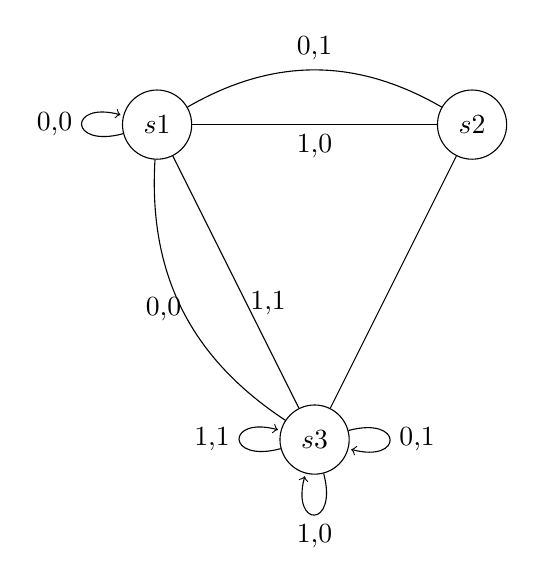
\begin{tikzpicture}
	% tikz code goes here
	\node[state] (s1) at (0, 4) {$s1$};
	\node[state] (s2) at (4, 4) {$s2$};
	\node[state] (s3) at (2, 0) {$s3$};
	\draw	(s1) edge[loop left] node{0,0} (s1)
			(s1) edge[bend left, above] node{0,1} (s2)
			(s1) edge[below] node{1,0} (s2)
			(s1) edge[below] node{\ \ \ \ \ \ \ 1,1} (s3)
			(s2) edge[below] node{} (s3)
			(s3) edge[loop left] node{1,1} (s3)
			(s3) edge[loop below] node{1,0} (s3)
			(s3) edge[loop right] node{0,1} (s3)
			(s3) edge[bend left] node{0,0\ \ \ \ \ } (s1);
	\end{tikzpicture}
	\caption{A state transition diagram.}
	\label{fig:my_label}
\end{figure}

\newpage
\section[20pt]{Finite-State Machines in Sequence Detection}
Finite-state machines can be used to detect sequences of numbers. To simplify, this paper will only be studying finite-state machines that detect sequences of 0s and 1s. This also gives the finite-state machines a digital analog. Consider the following example.
\newline
\newline
Ex. A system is given an a semi-random input stream of 0s and 1s. 10111100111000101 Draw a state transition diagram that detects if and when the sequence "110" appears when iterating through the input stream.
\begin{figure}[ht]
	\centering
	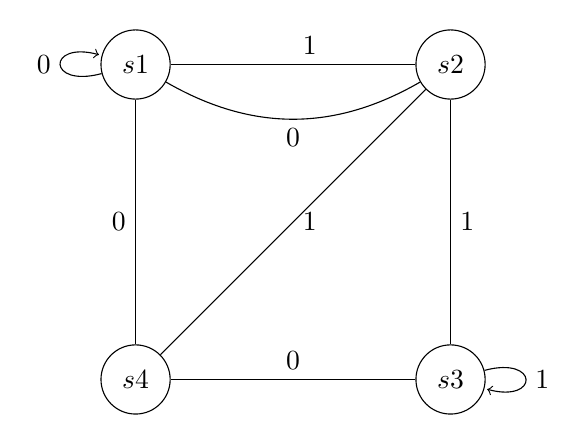
\begin{tikzpicture}
	\node[state] (s1) at (0, 4) {$s1$};
	\node[state] (s2) at (4, 4) {$s2$};
	\node[state] (s3) at (4, 0) {$s3$};
	\node[state] (s4) at (0, 0) {$s4$};
	\draw  (s1) edge[loop left] node{0} (s1)
	       (s1) edge[above right] node{1} (s2)
	       (s2) edge[below, bend left] node{0} (s1)
	       (s2) edge[right] node{1} (s3)
	       (s3) edge[loop right] node{1} (s3)
	       (s3) edge[above] node{0} (s4)
	       (s4) edge[left] node{0} (s1)
	       (s4) edge[right] node{1} (s2);
	\end{tikzpicture}
	\caption{Sequence "110" detector.}
\end{figure}
\newline
In Figure 2, s1 represents the initial state of the state-machine. When the state-machine gets a new input, it follows the corresponding arrow to the corresponding state. Reaching the final state, s4 represents the system successfully detecting "110". We will call these state-machines detectors.
\newline
\newline
Intuitively, every three-bit sequence will have its own unique detector. Each detector is a directed graph with very special properties. However, any given directed graph with 4 vertices will almost certainly not be a detector for any 3-bit sequence. There are 8 possible 3-bit sequences. In contrast, there are an infinite number of possible directed graphs with 4 vertices! The list of conditions for directed graphs to be a detector is very steep. One can compile a list of conditions a directed graph will need to satisfy to become a "detector", and in this way, an isomorphism can be established between binary numbers and the set of all "detector" graphs.
\newpage
\section[20pt]{Properties of Detectors}
\textbf{Definition 1.1}. A \textbf{detector} is a directed graph defined by a sequence of 0s and 1s, an initial vertex, and a final vertex. Progression through the graph is possible, by referring to a series of 1 bit binary inputs. The final vertex is reached if and only if that sequence of inputs appear.
\newline
\newline
\textbf{Theorem 1.1}. An n-bit detector has exactly n+1 vertices.
\newline
\textbf{Proof}. Consider an n-bit detector. \newline
The detector must have an initial vertex. (Def. 1.1) \newline
Progress to the final vertex can be measured discretely by starting at the front of the input sequence and counting how many bits are matched by the detector sequence. For each discrete step of progression, one vertex must be defined. Since the detector sequence is n-bit, n progression vertices must be defined. \newline
Thus, the number of all vertices in an n-bit detector-the initial and the progression vertices-is n + 1. \newline
\(\blacksquare\) \newline
\newline
\textbf{Theorem 1.2} An n-bit detector has 2n edges. \newline
\textbf{Proof}. Consider an n-bit detector. \newline
The detector must have n vertices. (Thm. 1.1) \newline
The input sequence is binary (Def. 1.1) so each vertex has exactly 2 edges coming out. Thus, an n-bit detector has 2n edges. \newline
\(\blacksquare\) \newline
\newline
\begin{figure}[ht]
	\centering
	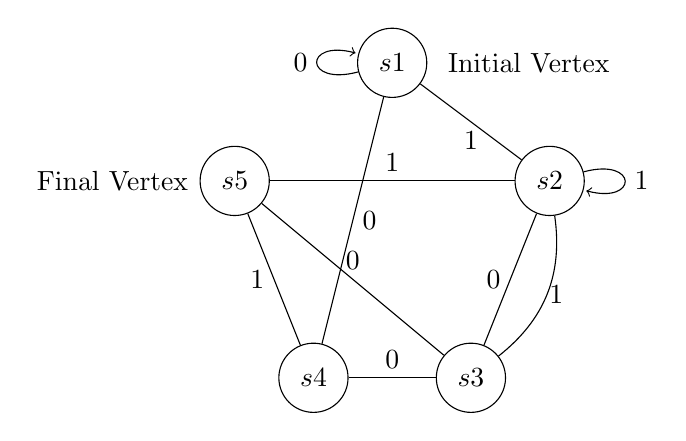
\begin{tikzpicture}
	\node[state] (s1) at (2, 4) {$s1$};
	\node[state] (s2) at (4, 2.5) {$s2$};
	\node[state] (s3) at (3, 0) {$s3$};
	\node[state] (s4) at (1, 0) {$s4$};
	\node[state] (s5) at (0, 2.5) {$s5$};
	\node[right] at (s1) {\ \ \ \ \ Initial Vertex};
	\draw  (s1) edge[loop left] node{0} (s1)
		   (s1) edge[below] node{1} (s2)
		   (s2) edge[left] node{0} (s3)
		   (s2) edge[loop right] node{1} (s2)
		   (s3) edge[above] node{0} (s4)
		   (s3) edge[bend right] node{\ \ 1} (s2)
		   (s4) edge[right] node{0} (s1)
		   (s4) edge[left] node{1} (s5)
		   (s5) edge[above] node{1} (s2)
		   (s5) edge[above] node{0} (s3);
	\node[left] at (s5) {Final Vertex\ \ \ \ \ };
	\end{tikzpicture}
	\caption{Sequence "1001" detector.}
\end{figure}
\newline
Note that the 4-bit detector shown in Figure 3 has 5 vertices. s1 is the initial vertex, while s2, s3, s4, and s5 are the progression vertices. Also note that the Figure has 10 edges, where each vertex has 2 pointing.
\newpage
\section[20pt]{Properties of Detectors cont.}
\textbf{Theorem 1.3} Every vertex \(s_k\) in an n-bit detector, except for \(s_n\), has one output going to \(s_k+1\) and one output going to a some vertex \(s_h\) where \(0\leq h\leq k\)\newline
\textbf{Proof}. Consider a k-bit detector defined with some sequence of bits \(b_0b_1...b_{k-1}\)
\newline
\begin{figure}[ht]
	\centering
	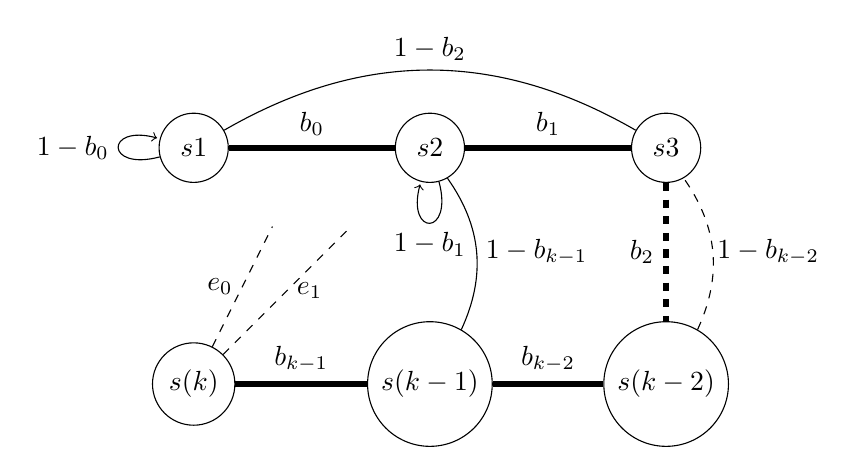
\begin{tikzpicture}
	\node[state] (s1) at (0,3) {$s1$};
	\node[state] (s2) at (3,3) {$s2$};
	\node[state] (s3) at (6,3) {$s3$};
	\node[state] (s4) at (6,0) {$s(k-2)$};
	\node[state] (s5) at (3,0) {$s(k-1)$};
	\node[state] (s6) at (0,0) {$s(k)$};
	
	\draw (s1) edge[loop left] node{\(1-b_0\)} (s1)
	      (s1) edge[above, line width = 2pt] node{\(b_0\)} (s2)
	      (s2) edge[loop below] node{\(1-b_1\)} (s2)
	      (s2) edge[above, line width = 2pt] node{\(b_1\)} (s3)
	      (s3) edge[bend right, above] node{\(1-b_2\)} (s1)
	      (s3) edge[left, dashed, line width = 2pt] node{\(b_2\)} (s4)
	      (s4) edge[above, line width = 2pt] node{\(b_{k-2}\)} (s5)
	      (s4) edge[bend right, dashed] node{\ \ \ \ \ \ \ \ \ \ \ \ \(1-b_{k-2}\)} (s3)
	      (s5) edge[above, line width = 2pt] node{\(b_{k-1}\)} (s6)
	      (s5) edge[bend right] node{\ \ \ \ \ \ \ \ \ \ \ \ \ \(1-b_{k-1}\)} (s2)
	      (s6) edge[left, dashed] node{\(e_0\)} (1,2)
	      (s6) edge[right, dashed] node{\(e_1\)} (2,2);
	\end{tikzpicture}
	\caption{Some k bit detector.}
\end{figure}
\newline
In order to detect the sequence, we need a the sequence of edges \(b_0,b_1,b_2...b_{k-2},b_{k-1}\) to chain the first vertex, s1 to the final vertex s(k). \newline
By Def. 1.1, each vertex has two edges coming out of it. With one edge taken care of, each vertex has one free edge to go to another vertex. \newline
This free edge cannot connect to any be directed at any vertex further down. This would allow the detector to reach the final state in less than k steps. Thus, the second edge of each vertex must be directed at either itself or a previous vertex. \newline
\(\blacksquare\) \newline
\newline
\textbf{Theorem 1.4} A detector has exactly 2 loops \newline
\textbf{Proof}. Consider an n-bit detector. \newline

\newpage
\section[20pt]{References}
(1) “Finite-State Machines.” Digital Design: an Embedded Systems Approach Using Verilog, by Peter J. Ashenden, Morgan Kaufmann, 2008, pp. 179–185.

\end{document}